\documentclass[11pt,letterpaper]{article}

\usepackage[margin=1in]{geometry}
\usepackage{minted}
\usepackage{graphicx}
\usepackage{hyperref}
\usepackage{titlesec}
\usepackage{fancyhdr}
\usepackage{xcolor}
\usepackage{caption}

\hypersetup{
    colorlinks=true,
    linkcolor=blue!60!black,
    bookmarksopen=true,
}

\pagestyle{fancy}
\fancyhf{}
\fancyhead[L]{\texttt{final\_project/fp}}
\fancyhead[R]{\thepage}
\renewcommand{\headrulewidth}{0.4pt}

\setminted{
    style=friendly,
    fontsize=\small,
    linenos=true,
    breaklines=true,
    frame=single,
    framesep=4pt,
    numbersep=6pt,
}

\titleformat{\section}{\large\bfseries}{}{0em}{}[\titlerule]

\title{\textbf{Grand Challenge --- Source Code Listing}\\[0.5em]
       \large ENPM 701}
\author{Marcus Hurt \\ \href{mailto:mhurt@umd.edu}{mhurt@umd.edu}}
\date{May 2026}

\begin{document}

\maketitle
\tableofcontents
\clearpage

% ── Robot path figures ────────────────────────────────────────────────────────

\section{Robot Path Plots}

\begin{figure}[h]
    \centering
    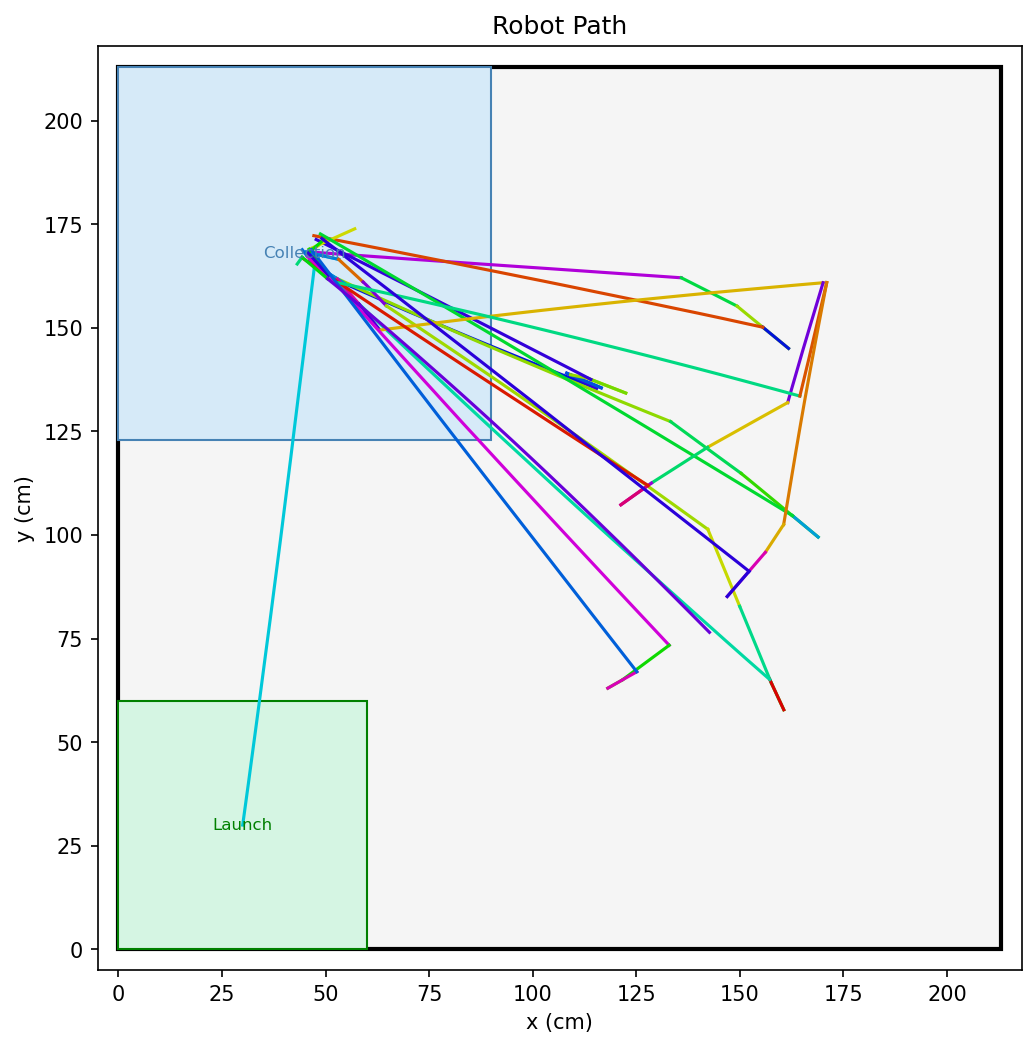
\includegraphics[width=0.85\textwidth]{run_1.png}
    \caption{Robot path --- Run 1}
\end{figure}

\begin{figure}[h]
    \centering
    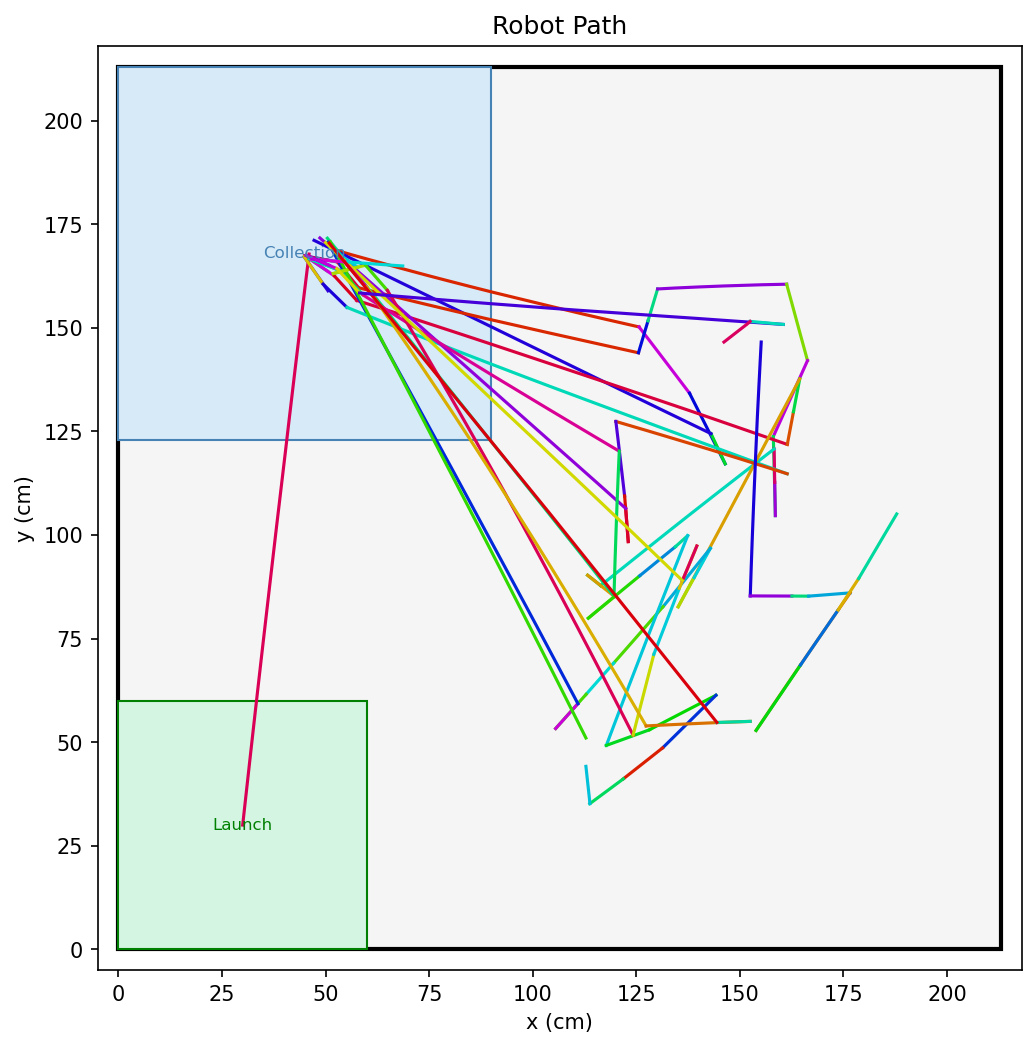
\includegraphics[width=0.85\textwidth]{run_2.png}
    \caption{Robot path --- Run 2}
\end{figure}

\clearpage

% ── Source files ──────────────────────────────────────────────────────────────

\section{\texttt{\_\_init\_\_.py}}
\inputminted{python}{fp/__init__.py}

\section{\texttt{\_\_main\_\_.py}}
\inputminted{python}{fp/__main__.py}

\section{\texttt{cli.py}}
\inputminted{python}{fp/cli.py}

\section{\texttt{arena.py}}
\inputminted{python}{fp/arena.py}

\section{\texttt{hal.py}}
\inputminted{python}{fp/hal.py}

\section{\texttt{motion.py}}
\inputminted{python}{fp/motion.py}

\section{\texttt{vision.py}}
\inputminted{python}{fp/vision.py}

\section{\texttt{localization.py}}
\inputminted{python}{fp/localization.py}

\section{\texttt{mapping.py}}
\inputminted{python}{fp/mapping.py}

\section{\texttt{search.py}}
\inputminted{python}{fp/search.py}

\section{\texttt{fsm.py}}
\inputminted{python}{fp/fsm.py}

\end{document}
